\documentclass[aspectratio=169, dvipdfmx, 11pt]{beamer} % aspectratio=43, 149, 169
\usepackage{here, amsmath, latexsym, amssymb, bm, ascmac, mathtools, multicol, tcolorbox, subfig}

%デザインの選択(省略可)
\usetheme{Luebeck}
%カラーテーマの選択(省略可)
\usecolortheme{orchid}
%フォントテーマの選択(省略可)
\usefonttheme{professionalfonts}
%フレーム内のテーマの選択(省略可)
\useinnertheme{circles}
%フレーム外側のテーマの選択(省略可)
\useoutertheme{infolines}
%しおりの文字化け解消
\usepackage{atbegshi}
\ifnum 42146=\euc"A4A2
\AtBeginShipoutFirst{\special{pdf:tounicode EUC-UCS2}}
\else
\AtBeginShipoutFirst{\special{pdf:tounicode 90ms-RKSJ-UCS2}}
\fi
%ナビゲーションバー非表示
\setbeamertemplate{navigation symbols}{}
%既定をゴシック体に
\renewcommand{\kanjifamilydefault}{\gtdefault}
%タイトル色
\setbeamercolor{title}{fg=structure, bg=}
%フレームタイトル色
\setbeamercolor{frametitle}{fg=structure, bg=}
%スライド番号のみ表示
%\setbeamertemplate{footline}[frame number]
%itemize
\setbeamertemplate{itemize item}{\small\raise0.5pt\hbox{$\bullet$}}
\setbeamertemplate{itemize subitem}{\tiny\raise1.5pt\hbox{$\blacktriangleright$}}
\setbeamertemplate{itemize subsubitem}{\tiny\raise1.5pt\hbox{$\bigstar$}}

% color
\newcommand{\red}[1]{\textcolor{red}{#1}}
\newcommand{\green}[1]{\textcolor{green!40!black}{#1}}
\newcommand{\blue}[1]{\textcolor{blue!80!black}{#1}}

\usepackage{hyperref}

% フレームのタイトル部分のフォントサイズを設定
\setbeamerfont{frametitle}{size=\huge}

\title[さんかく]{\Huge 自己紹介}
%\subtitle{副題}
\author[Zenn: \href{https://zenn.dev/joho0724}{@joho0724}]{\Large さんかく}
\institute[Qiita: \href{https://qiita.com/triangle0724}{@triangle0724}]{\large Zenn: \href{https://zenn.dev/joho0724}{@joho0724}}
\date{\today}

\begin{document}
\maketitle

\begin{frame}
    \frametitle{プロフィール}
    \begin{minipage}[t]{0.35\textwidth}
      \vspace{0pt}
      \centering
      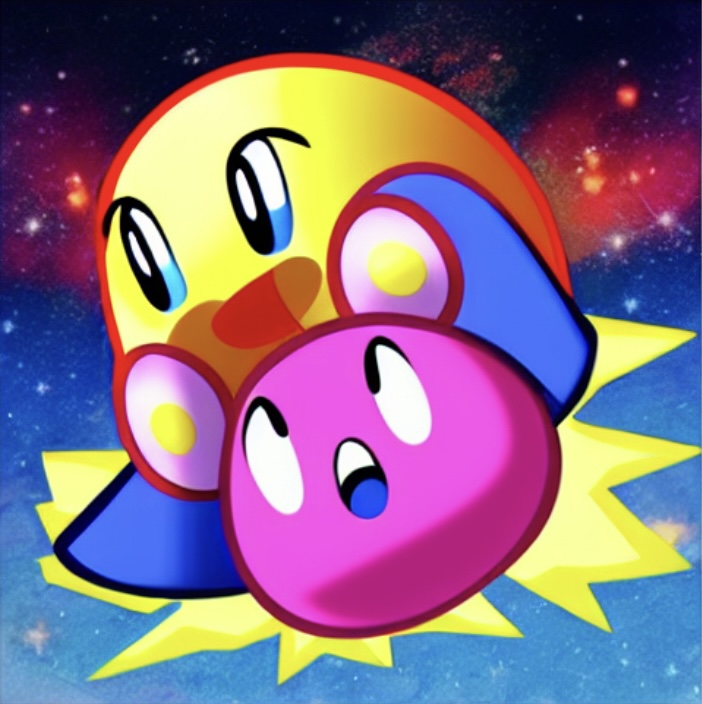
\includegraphics[width=1.0\linewidth]{fig/triangle.jpg}\\
    \end{minipage}
    \begin{minipage}[t]{0.65\textwidth}
      \vspace{0pt}
      \hspace{0.5cm} % 文章を右にずらす
      \huge
      さんかく
      \vspace{0.5cm} % スペースの追加
      \LARGE
      \begin{itemize}
        \item 年齢:22歳
        \item 出身地:広島県
        \item 誕生日:7月24日
        \item 血液型:B
        \item 座右の銘:一寸の光陰軽んずべからず
    \end{itemize}
    \end{minipage}
\end{frame}

\begin{frame}
    \frametitle{趣味}
    \begin{minipage}[t]{0.4\textwidth} % 左側の minipage の幅を調整
      \vspace{0pt}
      \centering
      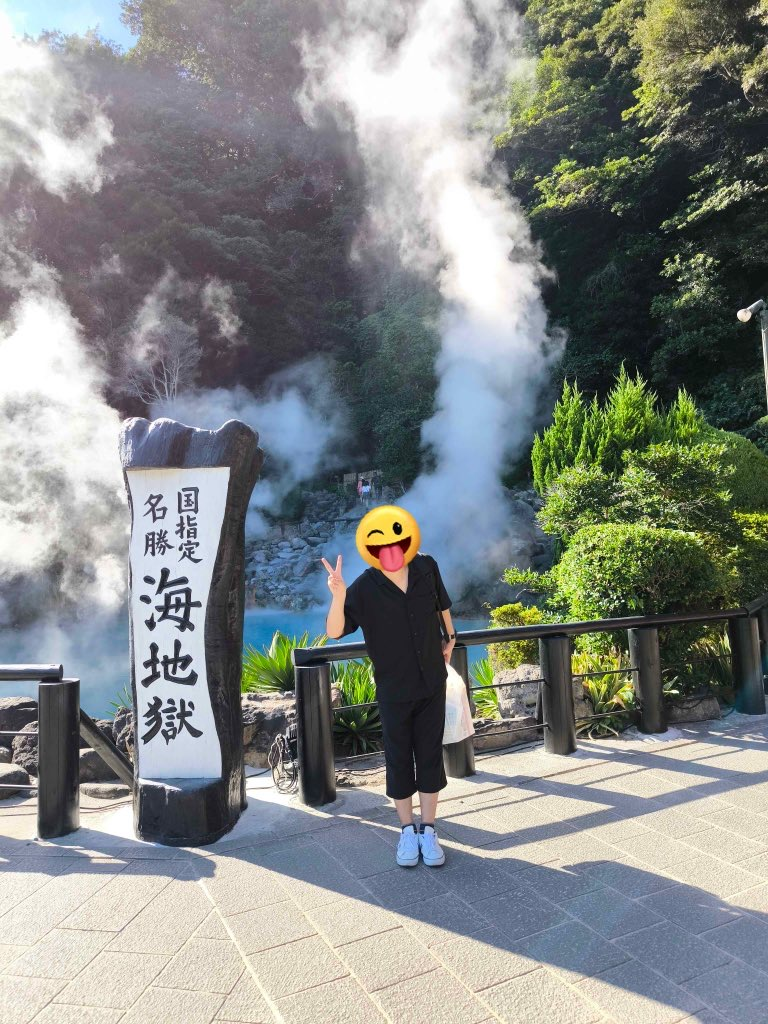
\includegraphics[width=0.8\linewidth]{fig/umi.JPG}\\
    \end{minipage}%
    \begin{minipage}[t]{0.6\textwidth}
      \vspace{0pt}
      \hspace{0.5cm} % 文章を右にずらす
      \LARGE
      \begin{itemize}
        \item お好み焼きを作ること
        \begin{itemize}
            \item {\Large 広島風しか勝たん}
        \end{itemize}
        \item 3DSのすれちがい通信
        \begin{itemize}
            \item {\Large ピース集めの旅をしています}
        \end{itemize}
        \item カラオケ
        \begin{itemize}
            \item {\Large 米津玄師が好きです}
        \end{itemize}
        \item 人狼ゲーム
        \begin{itemize}
            \item {\Large 対面でもスマホアプリでも}
        \end{itemize}
    \end{itemize}
    \end{minipage}
\end{frame}

\begin{frame}{興味・関心事}
    \begin{minipage}[t]{0.3\textwidth}
      \vspace{0pt}
      \centering
      
\includegraphics[width=1.1\linewidth]{fig/kkrn_icon_internet_1.png}
    \end{minipage}%
    \begin{minipage}[t]{0.65\textwidth}
        \vspace{0pt}
        \hspace{0.5cm} % 文章を右にずらす
        \huge
        ネットワーク学んでます
        \vspace{0.5cm} % スペースの追加
        \LARGE
        \begin{itemize}
          \item メディアアクセス制御関連の研究してます
          \item その他の技術にも興味あり
          \item 知識を深めていきたい!
      \end{itemize}
      \end{minipage}
\end{frame}


\begin{frame}{おわり}
    \centering
    \Huge
    ご覧いただき、\\ありがとうございました!\\
    \vspace{0.5cm} % スペースの追加
    \normalsize
    \begin{flushleft}
    アカウント
    \begin{itemize}
        \item Website: \href{https://sankaku0724.github.io/}{https://sankaku0724.github.io/}
        \item Zenn: \href{https://zenn.dev/joho0724}{@joho0724}
        \item X: \href{https://twitter.com/triangle0724}{@triangle0724}
        \item Github: \href{https://github.com/sankaku0724}{@sankaku0724}
        \item Qiita: \href{https://qiita.com/triangle0724}{@triangle0724}
        \item \href{https://speakerdeck.com/sankaku0724}{Speaker Deck}
    \end{itemize}
\end{flushleft}
\end{frame}

\end{document}
